% Options for packages loaded elsewhere
\PassOptionsToPackage{unicode}{hyperref}
\PassOptionsToPackage{hyphens}{url}
\PassOptionsToPackage{dvipsnames,svgnames,x11names}{xcolor}
\documentclass[
  10pt,
  fontset=fandol]{ctexart}
\usepackage{xcolor}
\usepackage[margin=16mm]{geometry}
\usepackage{amsmath,amssymb}
\setcounter{secnumdepth}{-\maxdimen} % remove section numbering
\usepackage{iftex}
\ifPDFTeX
  \usepackage[T1]{fontenc}
  \usepackage[utf8]{inputenc}
  \usepackage{textcomp} % provide euro and other symbols
\else % if luatex or xetex
  \usepackage{unicode-math} % this also loads fontspec
  \defaultfontfeatures{Scale=MatchLowercase}
  \defaultfontfeatures[\rmfamily]{Ligatures=TeX,Scale=1}
\fi
\usepackage{lmodern}
\ifPDFTeX\else
  % xetex/luatex font selection
\fi
% Use upquote if available, for straight quotes in verbatim environments
\IfFileExists{upquote.sty}{\usepackage{upquote}}{}
\IfFileExists{microtype.sty}{% use microtype if available
  \usepackage[]{microtype}
  \UseMicrotypeSet[protrusion]{basicmath} % disable protrusion for tt fonts
}{}
\makeatletter
\@ifundefined{KOMAClassName}{% if non-KOMA class
  \IfFileExists{parskip.sty}{%
    \usepackage{parskip}
  }{% else
    \setlength{\parindent}{0pt}
    \setlength{\parskip}{6pt plus 2pt minus 1pt}}
}{% if KOMA class
  \KOMAoptions{parskip=half}}
\makeatother
\usepackage{graphicx}
\makeatletter
\newsavebox\pandoc@box
\newcommand*\pandocbounded[1]{% scales image to fit in text height/width
  \sbox\pandoc@box{#1}%
  \Gscale@div\@tempa{\textheight}{\dimexpr\ht\pandoc@box+\dp\pandoc@box\relax}%
  \Gscale@div\@tempb{\linewidth}{\wd\pandoc@box}%
  \ifdim\@tempb\p@<\@tempa\p@\let\@tempa\@tempb\fi% select the smaller of both
  \ifdim\@tempa\p@<\p@\scalebox{\@tempa}{\usebox\pandoc@box}%
  \else\usebox{\pandoc@box}%
  \fi%
}
% Set default figure placement to htbp
\def\fps@figure{htbp}
\makeatother
\setlength{\emergencystretch}{3em} % prevent overfull lines
\providecommand{\tightlist}{%
  \setlength{\itemsep}{0pt}\setlength{\parskip}{0pt}}
\usepackage{amsmath,amssymb,mathtools,needspace}
\xeCJKDeclareCharClass{CJK}{"2032,"0400->"04FF,"2160->"216B,"2460->"2473,"25A0,"25C7,"25CB,"25CF}
\IfFontExistsTF{Arial Unicode MS}{\xeCJKsetup{AutoFallBack=true}\setCJKfallbackfamilyfont{\CJKrmdefault}{Arial Unicode MS}}{}
\setcounter{secnumdepth}{0}
\setlength{\emergencystretch}{2em}
\allowdisplaybreaks
\usepackage{bookmark}
\IfFileExists{xurl.sty}{\usepackage{xurl}}{} % add URL line breaks if available
\urlstyle{same}
\hypersetup{
  pdftitle={最佳一次逼近多项式},
  colorlinks=true,
  linkcolor={Maroon},
  filecolor={Maroon},
  citecolor={Blue},
  urlcolor={Blue},
  pdfcreator={LaTeX via pandoc}}

\title{最佳一次逼近多项式}
\author{}
\date{}

\begin{document}
\maketitle

\subsubsection{3.2.3 最佳一次逼近多项式}\label{ux6700ux4f73ux4e00ux6b21ux903cux8fd1ux591aux9879ux5f0f}

定理 3.4给出了最佳逼近多项式 \(P(x)\) 的特性, 但要求出 \(P(x)\) 却相当困难. 下面先讨论 \(n=1\) 的情形.

假定 \(f(x) \in C^2[a,b]\), 且 \(f''(x)\) 在 \((a,b)\) 内不变号, 要求最佳一次逼近多项式

\href{../../source-images/pdf-064.jpeg}{查看原页}

\(P_1(x) = a_0 + a_1x\). 根据定理3.4可知，至少有3个点 \(a \leqslant x_1 < x_2 < x_3 \leqslant b\)，使 \(P_1(x_k) - f(x_k) = (-1)^k \sigma \max_{a \leqslant x \leqslant b} |P_1(x) - f(x)|\) (\(\sigma = \pm 1, k = 1, 2, 3\)).

由于 \(f''(x)\) 在 \([a, b]\) 上不变号，故 \(f'(x)\) 单调，\(f'(x) - a_1\) 在 \((a, b)\) 内只有一个零点，记作 \(x_2\)，于是 \(P_1'(x_2) - f'(x_2) = a_1 - f'(x_2) = 0\)，即 \(f'(x_2) = a_1\).

另外两个偏差点必在区间端点，即 \(x_0 = a, x_1 = b\)，且满足 \[
P_1(a) - f(a) = P_1(b) - f(b) = -[P_1(x_2) - f(x_2)] .
\] 由此得到 \[
\begin{cases} a_0 + a_1a - f(a) = a_0 + a_1b - f(b), \\ a_0 + a_1a - f(a) = f(x_2) - (a_0 + a_1x_2). \end{cases} \tag{3.2.6}
\]

解出 \[
a_1 = \frac{f(b) - f(a)}{b - a} = f'(x_2), \tag{3.2.7}
\] 代入式(3.2.6)，得 \[
a_0 = \frac{f(a) + f(x_2)}{2} - \frac{f(b) - f(a)}{b - a} \frac{a + x_2}{2}. \tag{3.2.8}
\]

这就得到最佳一次逼近多项式 \(P_1(x)\)，其几何意义如图3.3所示。直线 \(y = P_1(x)\) 与弦 \(MN\) 平行，且通过 \(MQ\) 的中点 \(D\)，其方程为 \[
y = \frac{1}{2}[f(a) + f(x_2)] + a_1\left(x - \frac{a + x_2}{2}\right).
\]

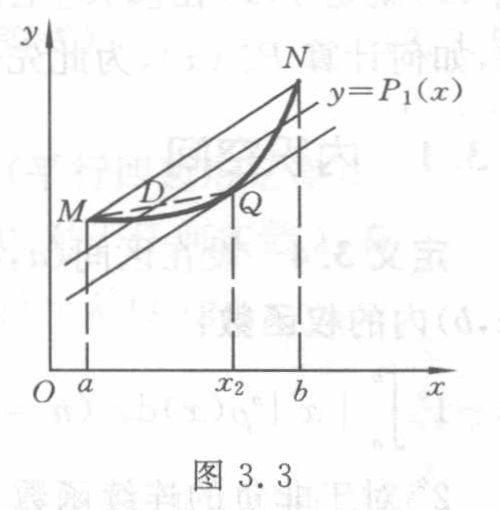
\includegraphics[width=0.85\linewidth,height=\textheight,keepaspectratio,alt={图 3.3 原图裁切}]{../assets/ch03a/fig-3-3.png}

图 3.3（原图）。最佳一次逼近的几何意义；标签为 \(x\)、\(y\)、\(O\)、\(a\)、\(x_2\)、\(b\)、\(M\)、\(N\)、\(Q\)、\(D\)、\(y=P_1(x)\)。弦 \(MN\)、逼近直线以及通过 \(Q\) 的平行线构成图中的三条斜线，\(D\) 为 \(MQ\) 的中点。

例3.1 求 \(f(x) = \sqrt{1+x^2}\) 在 \([0, 1]\) 上的最佳一次逼近多项式.

解 由式(3.2.7)可算出 \[
a_1 = \sqrt{2} - 1 \approx 0.414, \quad f'(x) = \frac{x}{\sqrt{1+x^2}},
\]

故 \[
\frac{x_2}{\sqrt{1+x_2^2}} = \sqrt{2} - 1,
\]

解得 \[
x_2 = \sqrt{\frac{\sqrt{2}-1}{2}} \approx 0.4551, \quad f(x_2) = \sqrt{1+x_2^2} \approx 1.0986.
\]

由式(3.2.8)，得 \[
a_0 = \frac{1 + \sqrt{1+x_2^2}}{2} - a_1 \frac{x_2}{2} \approx 0.955,
\]

于是得 \(\sqrt{1+x^2}\) 的最佳一次逼近多项式为 \[
P_1(x) = 0.955 + 0.414x,
\]

故 \[
\sqrt{1+x^2} \approx 0.955 + 0.414x, \quad 0 \leqslant x \leqslant 1. \tag{3.2.9}
\]

误差限为 \[
\max_{0 \leqslant x \leqslant 1} |\sqrt{1+x^2} - P_1(x)| \leqslant 0.045.
\]

\begin{quote}
校注（agent 补充，原书疑误）：本页开头先把三个交错点记为 \(x_1<x_2<x_3\)，随后原印``\(x_0=a,x_1=b\)''，此处忠实保留。按前文编号应为 \(x_1=a,x_3=b\)。
\end{quote}

\begin{quote}
校注（agent 补充，数值舍入）：原书对所写 \(P_1(x)=0.955+0.414x\) 给出误差限 \(0.045\)，这里保留原文。若把这两个已舍入系数当作精确数，则在 \(x=1\) 处误差为 \(\sqrt2-1.369\approx0.04521356>0.045\)，故所印误差限不适用于这组舍入后的系数。
\end{quote}

\href{../../source-images/pdf-065.jpeg}{查看原页}

在式(3.2.9)中若令 \(x = \frac{b}{a} \leqslant 1\), 则可得一个求根式的公式 \[
\sqrt{a^2 + b^2} \approx 0.955a + 0.414b.
\]

\subsection{本节覆盖原页的校注记录}\label{ux672cux8282ux8986ux76d6ux539fux9875ux7684ux6821ux6ce8ux8bb0ux5f55}

下列记录按原页关联，含同页相邻小节的校注；计算时同时读取上文校注和完整原页。

\begin{itemize}
\tightlist
\item
  \texttt{ch03a-E03}：原书 PDF 页 64
\item
  \texttt{ch03a-E04}：原书 PDF 页 64
\end{itemize}

\end{document}
